\documentclass{article}
\usepackage{iclr2026_conference,times} % ICLR 2027 submission using 2026 template

\usepackage{hyperref}
\usepackage{url}
\usepackage{amsmath,amssymb,amsfonts}
\usepackage{booktabs}
\usepackage{graphicx}
\usepackage{xcolor}
\usepackage{multirow}
\usepackage{enumitem}
\usepackage{subcaption}
\usepackage{amsthm}
\usepackage{microtype}
\newtheorem{proposition}{Proposition}

\newcommand{\ivs}{\text{IVS}}
\newcommand{\rest}{\text{Rest}}
\newcommand{\manifold}{\mathcal{M}}
\newcommand{\R}{\mathbb{R}}

\title{When Restoration Lies: Behavioral Effect Alone Is Insufficient Evidence \\
of Mechanism in Causal Interpretability}

\author{Anonymous}

\newcommand{\fix}{\marginpar{FIX}}
\newcommand{\new}{\marginpar{NEW}}

%\iclrfinalcopy
\begin{document}

\maketitle

\begin{abstract}
Activation patching is central to mechanistic interpretability, but a patch that restores the output need not be a valid mechanistic counterfactual. We argue that causal evidence from patching has at least three axes: behavioral restoration, intervention validity, and mechanism alignment. The missing axis is \emph{conditional validity}: whether the injected activation is plausible for the specific layer, position, and task condition being patched. We instantiate this axis with the Intervention Validity Score (IVS), a training-free conditional-overlap diagnostic, and use it to audit high-restoration interventions across transformer models. In seven IOI settings with both valid and invalid high-restoration patches, 22--42\% of patches are IVS-invalid; independent Name Mover Head validation on GPT-2 confirms that IVS-invalid patches often correspond to mechanism bypass (AUROC\,=\,0.89, zero false alarms). Mechanistically, these failures arise through answer smuggling: invalid patches restore the output while showing near-zero NMH recovery, large normal-manifold displacement, and alignment with the behavioral gradient. Conditioning is the core methodological requirement: same-site/same-context references separate valid and invalid patches, whereas mixed-site or wrong-position references collapse or invert the signal; among tested fixed diagnostics, IVS is the most stable implementation across architectures and hyperparameter regimes. Finally, repair experiments show a stricter hierarchy: restoring validity does not necessarily restore mechanism alignment. These results establish conditional intervention validity as a necessary diagnostic dimension for causal interpretability.
\end{abstract}

%=============================================================================
\section{Introduction}
\label{sec:intro}
%=============================================================================

Mechanistic interpretability often treats causal interventions as evidence about internal mechanisms. Activation patching, interchange interventions, causal tracing, and ablations modify hidden states and ask whether model behavior is restored \citep{vig2020investigating,meng2022locating,wang2022interpretability,geiger2024finding}. These tools are indispensable, but their evidential status is subtle: restoring behavior does not by itself show that the patched component is part of the mechanism.

This paper makes that caveat operational. We separate three evidence axes: \textbf{behavioral restoration} (whether the output is restored), \textbf{intervention validity} (whether the injected activation is plausible under the relevant layer/position/context), and \textbf{mechanism alignment} (whether the intended internal circuit is restored). The failure mode we study is a high-restoration intervention that is invalid under the conditional activation distribution. When independent circuit evidence also shows mechanism bypass, we call this a \emph{restoration lie}: the output is restored, but the patch did not restore the mechanism it appears to implicate.

Our central technical claim is that validity must be \emph{conditional}. An activation can be globally plausible while being implausible at the specific site and condition being patched. We therefore define validity relative to a site/context reference distribution and instantiate it with the Intervention Validity Score (IVS), a training-free diagnostic that combines local density, reconstruction error, and Mahalanobis fit. This separates the principle from the implementation: conditionality is the evidential requirement, and IVS is a stable fixed audit for applying it.

The empirical story follows the evidence hierarchy. First, behavioral restoration does not imply validity: across seven IOI settings with both valid and invalid high-restoration patches, 22--42\% of high-restoration patches are IVS-invalid. Second, invalid restoration is mechanistically meaningful rather than a scoring artifact: independent Name Mover Head (NMH) validation on GPT-2 shows that low-validity patches often bypass the intended IOI circuit rather than repairing it. Third, the diagnostic works for a principled reason: conditioning ablations show that generic OOD detection can erase or invert the signal. Finally, repair experiments sharpen the hierarchy by showing that even restored validity need not restore mechanism alignment.

Our contributions are: (1)~an evidence framework separating behavioral restoration, conditional intervention validity, and mechanism alignment; (2)~a multi-model IOI audit showing that invalid high-restoration interventions are common and independently associated with GPT-2 mechanism bypass; (3)~a mechanistic account of answer smuggling through normal displacement and late-layer shortcuts; (4)~IVS plus conditioning ablations showing that the reference distribution is the core design choice; and (5)~repair and clean-audit experiments sharpening the boundary between validity, mechanism alignment, and protocol. Appendix~\ref{app:evidence_map} summarizes the claim-evidence map.

%=============================================================================
\section{Background and Problem Formulation}
\label{sec:background}
%=============================================================================

\paragraph{Three axes of intervention evidence.}
Consider a transformer with $L$ layers and hidden dimension $d$. An intervention replaces activation $h_{l,p}$ at layer $l$, position $p$ with counterfactual $\tilde{h}_{l,p}$. We define three evidence axes:

\textbf{Behavioral effect} $E(\tilde{h}_{l,p})$ measures restoration of target behavior. For indirect object identification (IOI), this is the logit-difference restoration:
\begin{equation}
\rest(\tilde{h}_{l,p}) = \frac{\text{LD}_{\text{patched}} - \text{LD}_{\text{corrupt}}}{\text{LD}_{\text{clean}} - \text{LD}_{\text{corrupt}}}
\end{equation}

\textbf{Intervention validity} $V(\tilde{h}_{l,p})$ measures whether $\tilde{h}_{l,p}$ lies on the \emph{conditional} activation manifold $\manifold_{l,p}$---the set of activations the model would naturally produce at $(l, p)$ under the task condition. A valid intervention substitutes a plausible counterfactual; an invalid one injects an activation the model could never naturally produce at that site.

\textbf{Mechanism alignment} $A(\tilde{h}_{l,p})$ measures whether the intended internal mechanism is restored. In IOI, we instantiate $A$ as Name Mover Head (NMH) attention recovery: a patch is mechanism-aligned only if it restores both the output and the attention pathway that copies the indirect-object name.

Standard methodology measures only $E$. Our core claim is a hierarchy: $E$ does not imply $V$, and $V$ does not imply $A$. High-$E$, low-$V$ interventions---restoration lies---systematically mislead causal analysis; high-$V$, low-$A$ interventions show that validity is necessary but not sufficient for mechanistic correctness. Geometrically, $V$ tests membership in the conditional manifold $\manifold_{l,p}$, while $A$ tests membership in a stricter \emph{mechanism fiber}: the subset of that manifold that realizes the intended circuit state.

\paragraph{Why conditioning matters.}
The conditional nature of validity is essential. An activation may appear plausible in the global distribution of all model activations while being wildly implausible at a specific (layer, position). Section~\ref{sec:detection} demonstrates that unconditional Mahalanobis distance is weak for recovering validity labels, while conditional density estimators are much more reliable.

\paragraph{Related work.}
Activation patching \citep{vig2020investigating,meng2022locating}, interchange interventions \citep{geiger2024finding}, and path patching \citep{wang2022interpretability} use behavioral effect as the primary signal. Most related is \citet{grant2026addressing}, who showed that interventions can produce OOD states and proposed a contrastive training-time fix. Grant et al. identify a representation-validity problem; we show how conditional invalidity becomes a \emph{causal-evidence failure}: high restoration can support the wrong mechanism claim. The differences are concrete: validity is site/context conditional rather than global OOD \citep{lee2018simple}; invalid interventions are validated against independent NMH mechanism evidence rather than representation divergence alone; and IVS is a per-intervention, training-free audit for existing patching, ablation, and causal-tracing results rather than a training objective.

%=============================================================================
\section{Discovery: Conditional Validity Failures in High-Restoration Patches}
\label{sec:discovery}
%=============================================================================

We study IOI \citep{wang2022interpretability} across eight transformers in TransformerLens \citep{nanda2022transformerlens}, using five prompt templates and $N$=100--150 reference activations per site. For each high-restoration site ($>$10\%), we compute the Intervention Validity Score (IVS; formally defined in Section~\ref{sec:detection}).

\begin{table}[t]
\caption{IVS-invalid high-restoration patches across architectures on IOI. The gap ratio is $\min(\text{IVS}_\text{valid}) / \max(\text{IVS}_\text{invalid})$ when both classes are present. Site/gap columns are canonical full-batch or multi-template runs; bracketed 95\% CIs are available only for GPT-2, GPT-2 Medium, and Pythia-410M from 1{,}000 bootstrap resamples over 5 seeds $\times$ 5 templates. Independent mechanism-level validation is reported separately in Table~\ref{tab:independent}.}
\label{tab:gap}
\vspace{-2mm}
\begin{center}\small
\begin{tabular}{lccccc}
\toprule
\textbf{Model} & \textbf{Params} & \textbf{Sites} & \textbf{Invalid Rate} & \textbf{Gap} & \textbf{Border.} \\
\midrule
GPT-2 & 124M & 71 & 22.5\% [21.7, 23.4] & $2.8{\times}10^{12}$ & 0 \\
GPT-2 Med & 355M & 159 & 25.0\% [24.1, 25.8] & $2.9{\times}10^{12}$ & 0 \\
Pythia-410M & 410M & 172 & 34.2\% [28.1, 39.4] & $2.7{\times}10^{12}$ & 0 \\
OPT-2.7B & 2.7B & 231 & 30.7\% & $2.8{\times}10^{12}$ & 0 \\
OPT-6.7B & 6.7B & 239 & 34.7\% & $2.9{\times}10^{12}$ & 0 \\
GPT-J-6B & 6B & 203 & 40.4\% & $2.2{\times}10^{9}$ & 0 \\
Qwen-7B & 7B & 235 & 41.7\% & $9.8{\times}10^{1}$ & 1 \\
Pythia-6.9B & 6.9B & 224 & 0.0\% & n/a & 53--55 \\
\midrule
\multicolumn{2}{l}{\textbf{Total}} & \textbf{1,534} & & & \\
\bottomrule
\end{tabular}
\end{center}
\vspace{-3mm}
\end{table}

\begin{figure}[t]
\centering
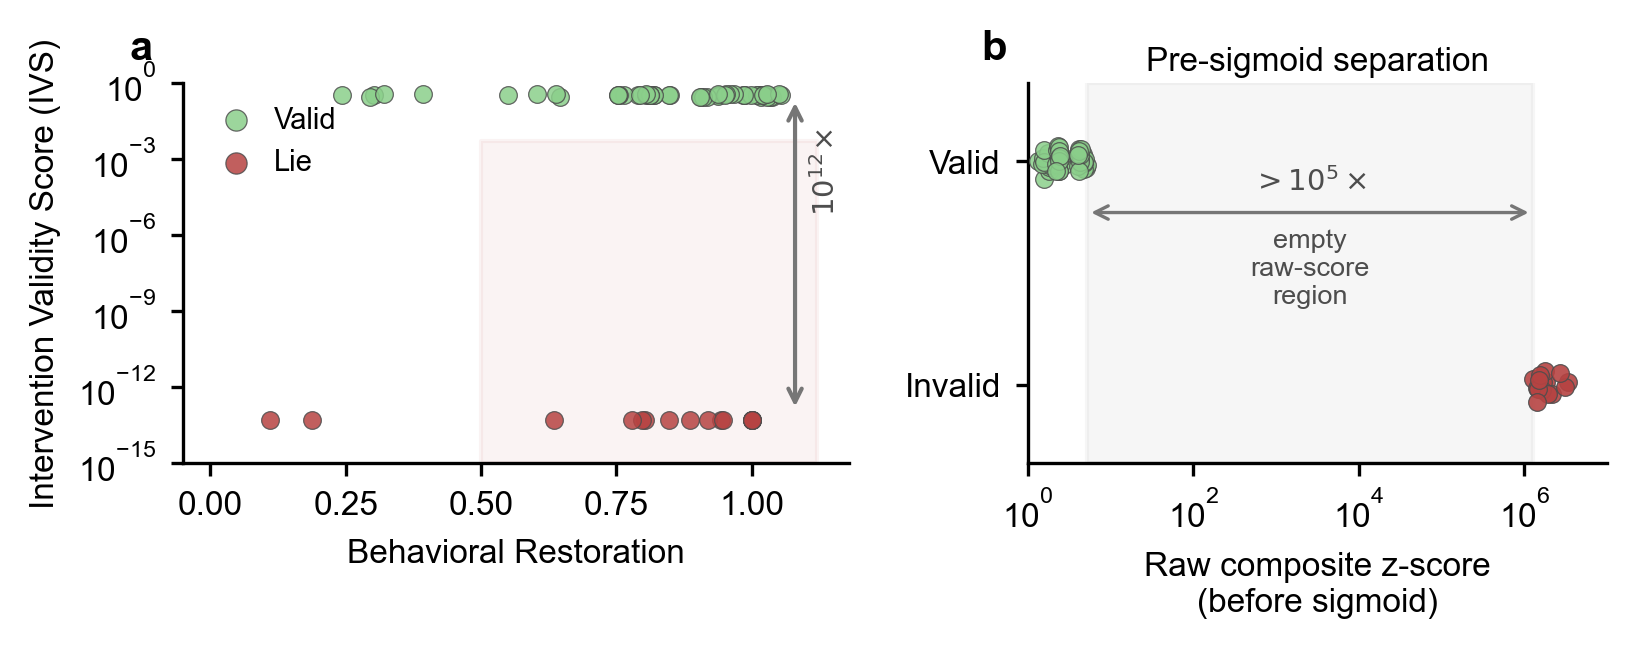
\includegraphics[width=0.96\linewidth]{figures/fig1_restoration_vs_ivs.pdf}
\vspace{-2mm}
\caption{\textbf{(a)} Restoration vs.\ conditional validity on GPT-2 IOI (71 sites, 5 templates). Valid patches (green) and IVS-invalid patches (red) achieve comparable restoration, but occupy sharply separated IVS regimes; the shaded region contains high-restoration interventions that restoration-only methodology would accept. \textbf{(b)} The separation is already present before the sigmoid mapping: raw composite z-scores for valid and invalid interventions are separated by an empty region spanning more than five orders of magnitude.}
\label{fig:scatter}
\vspace{-2mm}
\end{figure}

Table~\ref{tab:gap} and Figure~\ref{fig:scatter} present the central validity audit. For five models (GPT-2 through OPT-6.7B), high-restoration patches split into two sharply separated IVS regimes: valid sites have IVS\,$\in$\,[0.26, 0.40], while invalid sites sit near the numerical floor. This separation is not only a sigmoid artifact: before the sigmoid, the raw composite z-scores of valid sites lie in $[1.3, 5.2]$ while invalid sites range from $1.3{\times}10^{6}$ to $3.4{\times}10^{6}$, with a complete void spanning five orders of magnitude (Figure~\ref{fig:scatter}b; Appendix~\ref{app:zscore}). We therefore treat IVS as a conservative \emph{validity flag}: it identifies high-restoration interventions whose causal interpretation requires independent mechanism checks.

The separation magnitude varies systematically with architecture (Table~\ref{tab:gap}): models with absolute position embeddings (GPT-2, OPT) exhibit very hard boundaries, while RoPE-based GPT-J and Qwen exhibit smaller but still separable gaps. Pythia-6.9B is reported separately as a clean-audit case: two full-batch runs with $N_\text{ref}=150$ and 300 find 224 valid high-restoration sites and 0 invalid sites (Appendix~\ref{app:geometry_audit}). This sharpens the protocol claim: validity conclusions should be made under a precise patching protocol, and large-model implementation artifacts should be audited rather than folded into the main phenomenon.

These results establish that IVS-invalid restorations are common in several tested architectures (22--42\% of high-restoration patches). The next question is not merely whether these points are off-manifold, but whether they correspond to mechanistic failure. We therefore test \emph{why} invalid high-restoration patches work and \emph{where} they concentrate.

%=============================================================================
\section{Mechanism: Answer Smuggling and Phase Transition}
\label{sec:mechanism}
%=============================================================================

\subsection{Why lies work: answer smuggling}

We analyze the mechanism of restoration lies through Name Mover Head (NMH) attention recovery in GPT-2 on the IOI task \citep{wang2022interpretability}. The IOI circuit works by having NMHs attend to the indirect object name and copy it to the output. If a patch genuinely repairs the circuit, it should restore both the behavioral output \emph{and} the NMH attention pattern.

\begin{figure}[h]
\centering
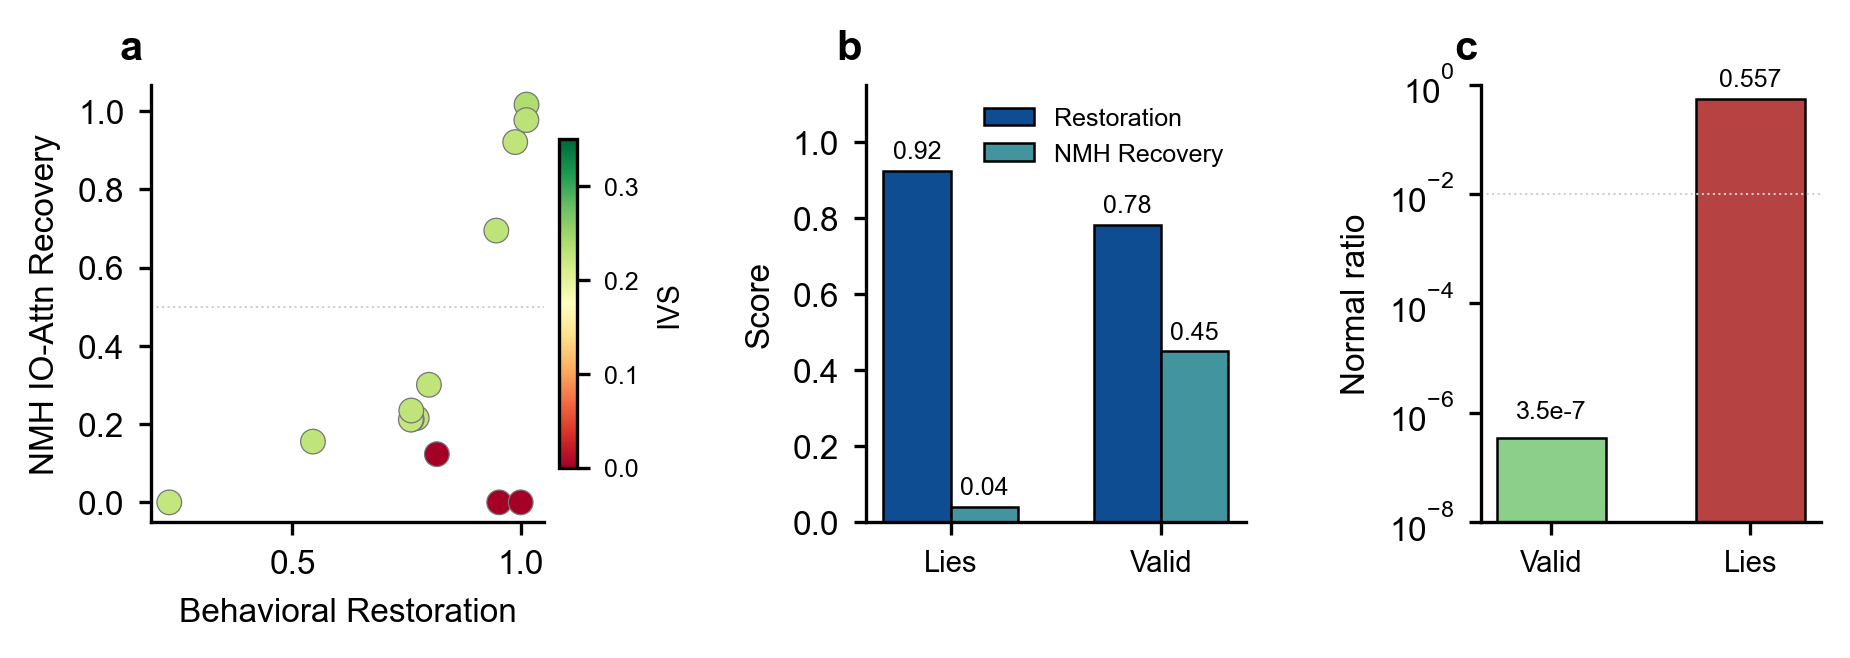
\includegraphics[width=\linewidth]{figures/fig4_answer_smuggling.pdf}
\vspace{-5mm}
\caption{Answer smuggling links mechanism failure to geometry. \textbf{(a)} Each site is colored by IVS. Low-IVS sites (red) achieve high restoration with near-zero NMH mechanism recovery, so they restore the answer without engaging the circuit. \textbf{(b)} Aggregated over GPT-2 high-restoration sites: last-token lies restore 92\% of behavior but only 4.1\% of NMH attention, whereas valid IO-position patches recover 44.9\% of NMH attention. \textbf{(c)} The same lies have large normal-manifold displacement (normal ratio 0.557 vs.\ $3.5{\times}10^{-7}$ for valid patches), showing that they are off-manifold shortcuts rather than circuit repairs.}
\label{fig:smuggling}
\vspace{-2mm}
\end{figure}

Figure~\ref{fig:smuggling} reveals the mechanism. Valid patches at the IO-name position (11 sites, layers 0--5) restore both logit difference \emph{and} NMH attention (44.9\% recovery). Lie patches at the last-token position (3 sites, layers 9--11) achieve 92\% behavioral restoration but only 4.1\% NMH recovery. These patches bypass the Name Mover circuit entirely by injecting the answer token's signal directly into the residual stream at a point close enough to the output that downstream processing simply passes it through---\emph{answer smuggling}.

The same conclusion holds geometrically. For each high-restoration site, we decompose the clean-corrupt displacement into the local PCA tangent subspace of the conditional reference manifold and its normal complement, then compare each component with the behavioral gradient. Valid patches have mean normal ratio $3.5{\times}10^{-7}$, whereas lies have mean normal ratio $0.557$ (Figure~\ref{fig:smuggling}c); the normal-gradient cosine is near zero for valid patches but $0.109$ for lies (Appendix~\ref{app:normal}). Thus lies are not generic outliers: they move substantially off the conditional manifold in a direction that is behaviorally effective.

This mechanism predicts a spatial pattern: lies should concentrate where the residual stream is close to the output, allowing direct signal injection.

\newpage
\subsection{Where lies occur: universal phase transition}

\begin{figure}[h]
\centering
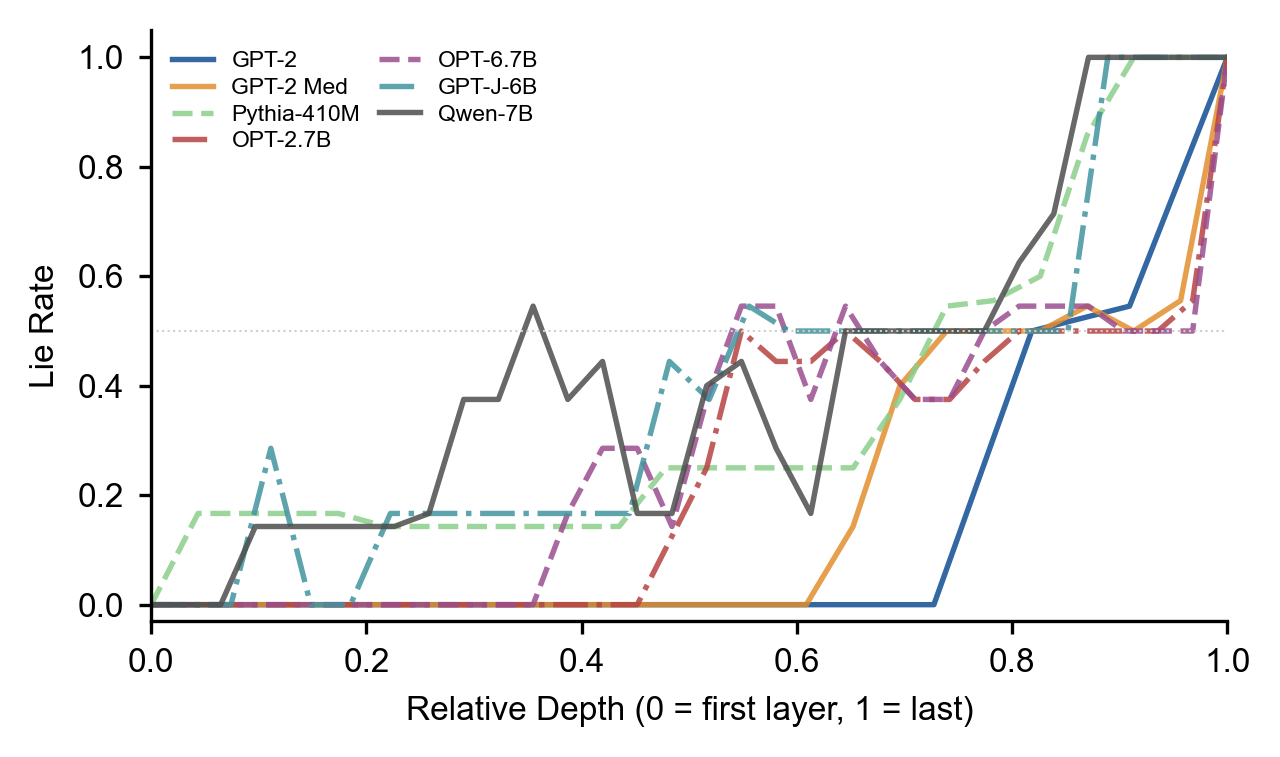
\includegraphics[width=0.78\linewidth]{figures/fig3_layer_transition.pdf}
\vspace{-2mm}
\caption{Layer-wise lie rate across seven architectures (124M--7B), normalized to relative depth. Lie rates are low or sparse in early layers, rise through middle/deep layers, and reach 100\% in the final layers, matching the answer-smuggling prediction.}
\label{fig:transition}
\vspace{-2mm}
\end{figure}

\begin{table}[h]
\caption{Phase transition locations across architectures. First-lie and all-lie depths are computed from the canonical layer-wise curves in Figure~\ref{fig:transition}.}
\label{tab:transition}
\vspace{-2mm}
\begin{center}\small
\setlength{\tabcolsep}{4pt}
\begin{tabular}{lccc}
\toprule
\textbf{Model} & \textbf{First Lie (\% depth)} & \textbf{All Lies (\% depth)} & \textbf{PE Type} \\
\midrule
GPT-2 & L9 (82\%) & L11 (100\%) & Absolute \\
GPT-2 Medium & L15 (65\%) & L23 (100\%) & Absolute \\
Pythia-410M & L1 (4\%) & L21 (91\%) & RoPE \\
OPT-2.7B & L15 (48\%) & L31 (100\%) & Absolute \\
OPT-6.7B & L12 (39\%) & L31 (100\%) & Absolute \\
GPT-J-6B & L3 (11\%) & L24 (89\%) & RoPE \\
Qwen-7B & L3 (10\%) & L27 (87\%) & RoPE \\
\bottomrule
\end{tabular}
\end{center}
\vspace{-3mm}
\end{table}

Figure~\ref{fig:transition} confirms this prediction across seven architectures. The common pattern is depth concentration: lie rates are low or sparse in early layers, rise through middle/deep layers, and reach 100\% in the final layers. The transition point varies by architecture (Table~\ref{tab:transition}), with GPT/OPT models showing especially late onsets and RoPE/Pythia-style models showing earlier sparse invalid sites.

The interpretation is straightforward: early-layer patches must propagate through many subsequent layers of genuine computation to affect the output, so only on-manifold activations succeed. Deep-layer patches are close to the output and can directly inject signal---\emph{any} activation with the right answer encoded will achieve high restoration regardless of manifold membership.

\subsection{Cross-task validation}

The phenomenon is not IOI-specific. Auditing ROME causal tracing \citep{meng2022locating} on GPT-2 and GPT-2~XL reveals that last-token patches are near-universally lies (100\% in GPT-2, 97.2\% in GPT-2~XL). Subject-token patches show a striking scaling effect: 67\% lies in GPT-2 (12 layers, 9 sites) but only 8.4\% in GPT-2~XL (48 layers, 381 sites)---the deeper model absorbs Gaussian corruption across more layers, making subject-position patches on-manifold by mid-depth (GPT-2~XL subject lies concentrate in layers 14--28, above 60\% relative depth). This yields a concrete cross-task lesson: \emph{causal tracing becomes substantially more reliable in larger models for subject-token interventions, but last-token patches remain dangerous regardless of scale}.

As a \textbf{negative control}, we audit GPT-2 induction heads \citep{olsson2022context}: all 28 high-restoration sites are valid (IVS\,$\in$\,[0.52, 0.76], lie rate\,=\,0\%). The corruption (token shuffle) preserves the sequence distribution, so all patches land on-manifold. IVS correctly identifies this as a clean setting, giving a simple specificity check: it flags invalid conditional interventions, not interventions indiscriminately. Full cross-task tables appear in Appendix~\ref{app:cross_task}.

The smuggling mechanism and phase transition explain \emph{when and where} independently validated restoration lies occur in GPT-2. The next question is broader: \emph{how can we audit conditional validity systematically, and what makes a good validity diagnostic?}

%=============================================================================
\section{Detection: Conditional Validity and IVS}
\label{sec:detection}
%=============================================================================

\subsection{Conditioning is the key insight}

We compare seven approaches for recovering the validity labels induced by a site/context conditional reference distribution (Table~\ref{tab:baselines}). The result is striking: \emph{all} conditional density estimators---those that score against the site-specific reference distribution $P_{l,p}$---separate valid from invalid GPT-2 patches perfectly. Unconditional methods are less reliable: global Mahalanobis achieves 0.555, barely above random. A trained MLP catastrophically overfits on 71 samples (AUROC\,=\,0.034 in the multi-template cross-validation protocol).

\begin{table}[t]
\caption{AUROC for recovering IVS-invalid validity labels on GPT-2 IOI (71 sites, 16 invalid patches). Conditional density estimation is sufficient for this validity audit; unconditional methods are less reliable. $^\dagger$MLP trains on 71 samples in $d$\,=\,768; the $d/N$\,=\,54.9 ratio causes catastrophic overfitting with inverted multi-template CV predictions (Appendix~\ref{app:baseline_audit}). Independent mechanism-level validation appears in Table~\ref{tab:independent}.}
\label{tab:baselines}
\vspace{-2mm}
\begin{center}\small
\begin{tabular}{lccc}
\toprule
\textbf{Method} & \textbf{AUROC} & \textbf{Cond.?} & \textbf{Train-free?} \\
\midrule
IVS (ours) & \textbf{1.000} & \checkmark & \checkmark \\
GMM density & 1.000 & \checkmark & \checkmark \\
KDE & 1.000 & \checkmark & \checkmark \\
One-Class SVM & 0.781 & \checkmark & \checkmark \\
Uncond.\ kNN & 0.898 & $\times$ & \checkmark \\
Uncond.\ Mahalanobis & 0.555 & $\times$ & \checkmark \\
Trained MLP$^\dagger$ (5-fold CV) & 0.034 & \checkmark & $\times$ \\
\bottomrule
\end{tabular}
\end{center}
\vspace{-3mm}
\end{table}

This reveals a crucial insight: \textbf{the innovation is conditioning, not the specific metric}. The fact that multiple conditional estimators agree on GPT-2 shows that invalid high-restoration patches are not an artifact of the IVS formula alone. At the same time, the MLP baseline illustrates why \emph{training-free} diagnostics are preferable in this setting: with $N$\,=\,71 samples in $d$\,=\,768 dimensions, a supervised learner is unstable under the multi-template CV protocol (Appendix~\ref{app:baseline_audit}).

A direct conditioning ablation confirms this interpretation (Appendix~\ref{app:conditionality}). On GPT-2, the correct same-site, same-context reference separates the validity labels perfectly. Mixing clean and corrupt contexts at the same site blurs the boundary (AUROC\,=\,0.71); mixing sites within the same layer nearly inverts the labels (AUROC\,=\,0.003); and using a wrong-position reference collapses both valid and invalid patches to the numerical floor. The same pattern appears on Pythia-410M: same-site/same-context separates the labels, while mixed-site/same-context drops to 0.012. Validity is therefore not generic OOD detection: it is a site- and context-conditional overlap property.

\subsection{A stable diagnostic for conditional validity}

If conditioning is the central idea, IVS is the fixed diagnostic that makes it practical without per-model training or detector tuning. GPT-2 is the easiest case: several conditional estimators separate the validity labels. On harder architectures, however, density estimators become more sensitive to bandwidth and mixture choices, while IVS remains stable across both hard and softer boundary regimes (Table~\ref{tab:cross_auroc}).

\begin{table}[t]
\caption{Cross-model AUROC for recovering conditional validity labels. IVS is the most stable diagnostic across both hard and softer boundary regimes. Pythia-6.9B is excluded from AUROC comparison because the clean full-batch audit yields no invalid class.}
\label{tab:cross_auroc}
\vspace{-2mm}
\begin{center}\small
\begin{tabular}{lcccc}
\toprule
\textbf{Model} & \textbf{Gap} & \textbf{IVS} & \textbf{GMM} & \textbf{KDE} \\
\midrule
GPT-2 & $10^{12}$ & 1.000 & 1.000 & 1.000 \\
Pythia-410M & $10^{12}$ & 1.000 & 1.000 & 0.509 \\
Qwen-7B & $10^{2}$ & \textbf{1.000} & 0.975 & 0.744 \\
\bottomrule
\end{tabular}
\end{center}
\vspace{-3mm}
\end{table}

On Qwen-7B, GMM drops to 0.975 and KDE to 0.744. GMM also has a hidden hyperparameter: although $n_\text{components}=1$ works on GPT-2 in the easy regime, larger mixture counts degrade substantially in the baseline audit (Appendix~\ref{app:baseline_audit}). Thus IVS does not claim uniqueness in the easy regime; it claims the stronger practical property: a fixed, training-free score that matches the best conditional estimators when separation is easy and remains strongest when the boundary softens. The separate Pythia-6.9B audit is a protocol boundary case, not a contradiction of the framework: once full-batch patching removes the invalid class, AUROC is no longer the right statistic; the correct report is that all 224 high-restoration sites are valid under two reference sizes. A visual summary of cross-architecture boundary sharpness appears in Appendix~\ref{app:boundary_visual}.

\subsection{IVS definition}

IVS is a training-free composite diagnostic. For each intervention site $(l, p)$, we collect a \emph{reference set} $\mathcal{R} = \{h_{l,p}(x_i)\}_{i=1}^{N}$ from $N$ forward passes under the corruption condition, project to a $k$-dimensional subspace via local PCA, and combine three complementary signals:
\begin{equation}
\text{IVS}(\tilde{h}) = \sigma\!\left(-\frac{z_\text{knn} + z_\text{recon} + z_\text{maha}}{3}\right)
\label{eq:ivs}
\end{equation}
where $z_\text{knn}$ is standardized kNN distance (local density), $z_\text{recon}$ is PCA reconstruction error (manifold membership), $z_\text{maha}$ is Mahalanobis distance (distributional fit), and $\sigma$ is the logistic sigmoid. IVS\,$\approx$\,0.3--0.4 indicates the activation is indistinguishable from natural ones; IVS\,$\approx$\,0 indicates a dramatic manifold violation.

Component ablations show that reconstruction error provides the strongest single signal, but the composite score is safer than any component alone: kNN alone assigns relatively high scores to last-position invalid patches, while full IVS drives them to the numerical floor (Appendix~\ref{app:component_intervention}).

\paragraph{Hyperparameter stability.}
IVS is stable over broad parameter ranges: lie rate remains 21.4\% for $k \in [5, 30]$, rank $\in [8, 64]$, and $N_\text{ref} \in [50, 300]$ on GPT-2. On the more challenging Pythia-70M, we recommend $k \geq 10$, rank $\geq 32$, $N_\text{ref} \geq 120$. The default configuration ($k$\,=\,12, rank\,=\,32, $N_\text{ref}$\,=\,150) works across all tested models without modification.

\subsection{Practical applications}

\paragraph{Intervention type audit.}
IVS reveals a practical finding with immediate implications: in our GPT-2 IOI audit, zero ablation---widely used as the default in circuit discovery \citep{conmy2023automated}---is invalid at every tested high-restoration site.

In this audit, the zero vector is not on the tested GPT-2 IOI conditional activation manifolds, while resample ablation stays valid by construction (Appendix~\ref{app:component_intervention}). This is a concrete practice-level consequence of conditional validity: circuits discovered via zero ablation should be re-validated with a distribution-preserving intervention.

\paragraph{IVS-guided patching eliminates circuit false positives.}
Invalid high-restoration patches produce concrete errors in circuit analysis. Across all five GPT-2 IOI templates, standard top-20 restoration ranking includes five L11/last-position smuggling sites (restoration\,$=$\,100\%, IVS\,$=$\,0), while IVS-guided ranking removes all five and recovers only L0--L3/IO-position sites from the known circuit \citep{wang2022interpretability}.

\begin{table}[h]
\caption{IVS-guided ranking removes restoration-only circuit false positives. Standard restoration ranking includes five deep last-token smuggling sites; validity filtering removes all five and recovers the known early IO-position circuit sites.}
\label{tab:ivs_guided_patching}
\vspace{-2mm}
\begin{center}
\small
\setlength{\tabcolsep}{5pt}
\begin{tabular}{lcccc}
\toprule
\textbf{Ranking} & \textbf{IO early} & \textbf{Deep last FP} & \textbf{Mean layer} & \textbf{Mean IVS} \\
\midrule
Standard top-20 & 15 & 5 & 3.5 & 0.249 \\
IVS-guided top-20 & \textbf{20} & \textbf{0} & 1.5 & 0.334 \\
\bottomrule
\end{tabular}
\end{center}
\vspace{-4mm}
\end{table}
Thus validity filtering is an actionable circuit-discovery filter (Table~\ref{tab:ivs_guided_patching}): it removes restoration-only smuggling sites and recovers the known circuit structure.

\subsection{Independent ground truth validation}
\label{sec:independent}

A potential concern is circularity: if lies are \emph{defined} by IVS\,$<$\,0.01, then IVS achieving high AUROC is tautological. We address this by evaluating IVS against a \textbf{completely independent} ground truth: Name Mover Head (NMH) attention recovery, which measures whether the downstream mechanism (not just the behavioral output) is restored.

For each of the 56 high-restoration sites across four GPT-2 templates, we compute both IVS and NMH IO-attention recovery. We define mechanism-bypassing sites as those with NMH recovery\,$<$\,20\%---a label derived entirely from attention patterns, with no dependence on IVS.

\begin{table}[h]
\caption{Independent validation: IVS evaluated against NMH-defined ground truth. IVS achieves AUROC\,=\,0.89 against an independent mechanism-level label with zero false alarms.}
\label{tab:independent}
\vspace{-2mm}
\begin{center}\small
\begin{tabular}{lccc}
\toprule
& \textbf{GPT-2} & \textbf{GPT-2 Med} \\
\midrule
High-restoration sites & 56 & 125 \\
NMH-bypass (nmh $<$ 0.20) & 16 & 38 \\
IVS-invalid (ivs $<$ 0.01) & 12 & 32 \\
\textbf{AUROC (IVS $|$ NMH)} & \textbf{0.894} & \textbf{0.778} \\
Agreement & 92.9\% & 84.0\% \\
IVS false alarms & 0 & 7 \\
IVS conservative misses & 4 & 13 \\
\bottomrule
\end{tabular}
\end{center}
\vspace{-3mm}
\end{table}

Table~\ref{tab:independent} shows that IVS achieves AUROC\,=\,0.89 on GPT-2 against NMH labels---the key non-circular validation result. On GPT-2 Medium (125 sites), AUROC is 0.78 because the seven IVS false alarms are all L15--L17 last-token transition sites with borderline NMH recovery (0.20--0.38); raising the NMH cutoff to 0.30/0.35 reduces them to 2/1 (Appendix~\ref{app:nmh_threshold}). Crucially, on GPT-2 \textbf{IVS produces zero false alarms}: every site IVS flags as invalid is independently confirmed as mechanism-bypassing by NMH. The 4 ``conservative misses'' are mid-depth IO-position sites where NMH recovery is low (0.18--0.21) but IVS rates them as marginally valid---IVS errs on the side of caution.

Detection naturally raises the final question: \emph{can invalid high-restoration patches be repaired to become valid interventions, and what does repair reveal about the manifold geometry?}

%=============================================================================
\section{Repair and Manifold Geometry}
\label{sec:repair_sec}
%=============================================================================

Repair experiments are not presented as a mechanism-repair method; they test the boundary between validity and mechanism alignment. kNN projection onto nearby reference activations restores validity for all tested invalid patches (9/9 GPT-2 and 39/39 OPT-2.7B), while tangent-space projection fails entirely; the appendix also shows a sharp IVS phase transition as repaired points are interpolated back toward the original invalid patch (Appendix~\ref{app:repair_details}). Thus valid counterfactuals exist near these patches, but the local manifold geometry is not captured by a linear tangent subspace alone.

The repair audit also establishes the second half of the R/V/A hierarchy: validity is necessary but not sufficient for mechanism alignment. On GPT-2, kNN repair raises IVS from the numerical floor to $\approx$0.27, but NMH recovery improves only from 3.6\% to 4.9\%, far below valid-patch recovery (44.9\%). Even a fiber-aware oracle over nearby reference activations raises IVS to 0.463--0.475 while leaving NMH alignment at only 3.7--4.2\% (Appendix~\ref{app:repair_details}). A valid intervention can therefore land on the right conditional manifold while still occupying the wrong mechanism fiber.

%=============================================================================
\section{Geometric Perspective}
\label{sec:theory}
%=============================================================================

The R/V/A hierarchy has a simple geometric interpretation. Behavioral restoration $R$ constrains only a level set of the output metric; intervention validity $V$ asks whether the injected activation lies in the thin conditional support $\manifold_{l,p}$; and mechanism alignment $A$ asks whether it lies in the smaller mechanism fiber that realizes the intended circuit state. In high dimension, satisfying the output level set does not imply landing in the conditional support, and landing in the support does not imply landing in the right fiber. The normal-direction audit, repair failure, and intrinsic-dimension estimates all support this picture; formal statements and proof sketches are deferred to Appendix~\ref{app:theory_details}.

%=============================================================================
\section{Discussion and Conclusion}
\label{sec:discussion}
%=============================================================================

\paragraph{Implications for existing work.}
Our finding that zero ablation is invalid at every tested GPT-2 IOI high-restoration site has immediate implications for circuit discovery \citep{conmy2023automated}. More broadly, the audits suggest that restoration-only patching results can include invalid deep-layer shortcuts. We do not claim prior conclusions are necessarily wrong---many may survive validity filtering---but that \textbf{intervention validity should be reported alongside behavioral effect} as standard practice.

\paragraph{Robustness and boundary cases.}
Bootstrap resampling over 5 seeds $\times$ 5 templates yields tight 95\% CIs for GPT-2 (22.5\% [21.7, 23.4]) and GPT-2~Medium (25.0\% [24.1, 25.8]), with no borderline cases in the hard-boundary models. The largest IVS gaps are sigmoid-amplified but not sigmoid-created: raw valid z-scores lie in $[1.3, 5.2]$ while invalid sites lie in $[1.3{\times}10^6, 3.4{\times}10^6]$ (Appendix~\ref{app:zscore}). Boundary cases sharpen the hierarchy: Pythia-6.9B is a clean-audit protocol case, kNN repair restores validity without restoring NMH alignment, and cross-task evidence supports generality while leaving IOI as the deepest audit.

\paragraph{Conclusion.}
Behavioral restoration alone is insufficient for mechanism claims: across IOI architectures, 22--42\% of high-restoration patches are IVS-invalid, and in GPT-2 these invalid patches independently align with NMH mechanism bypass. The resulting evidence tuple is restoration, intervention validity, and mechanism alignment.

\clearpage
\bibliography{references}
\bibliographystyle{iclr2026_conference}

\clearpage
\appendix

\section{Boundary and Repair Visualizations}
\label{app:boundary_visual}

\begin{figure}[h]
\centering
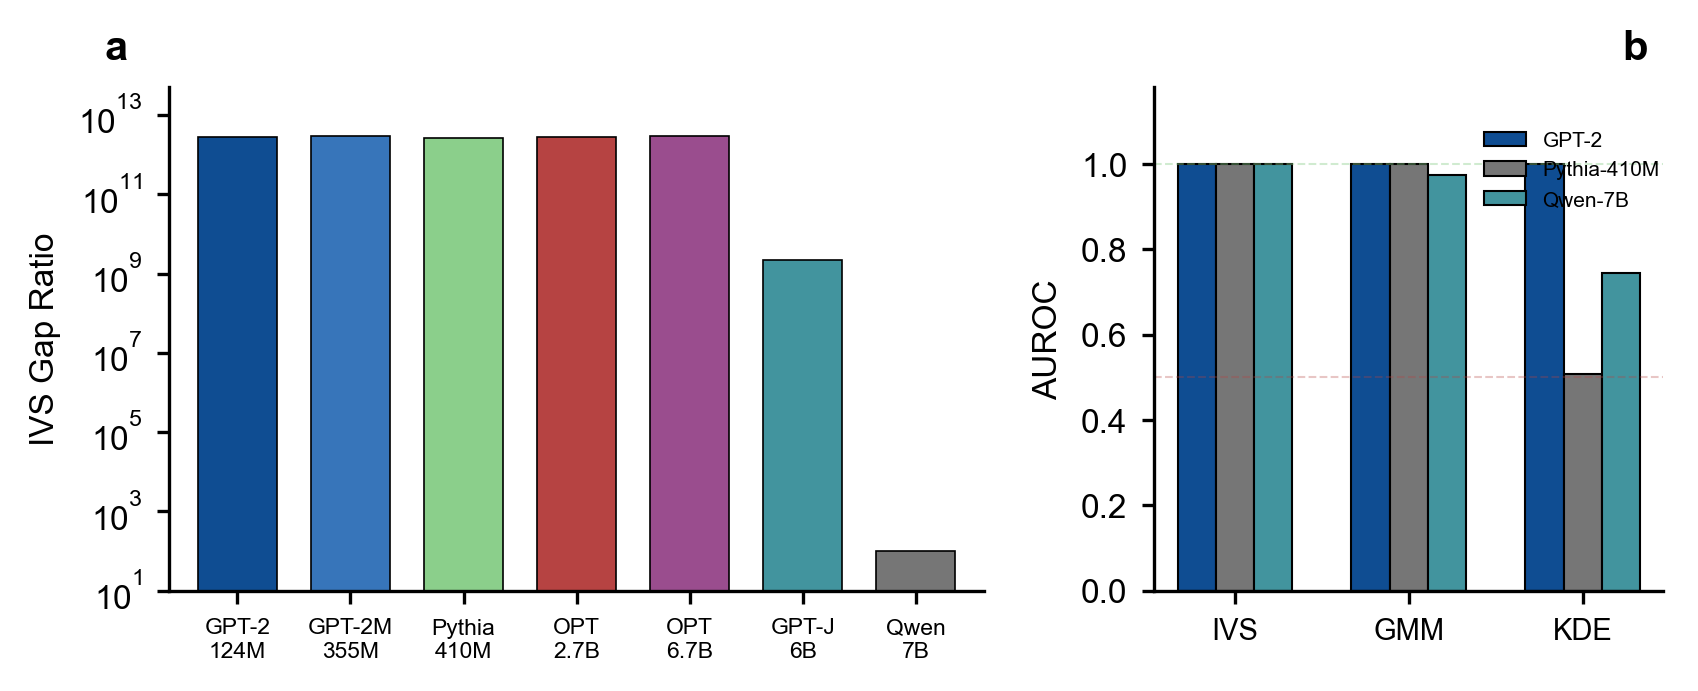
\includegraphics[width=\linewidth]{figures/fig5_boundary_sharpness.pdf}
\caption{\textbf{(a)} IVS gap across architectures with both valid and invalid sites (log scale). Gap varies from very hard (GPT-2/OPT) to softer but still separable (Qwen); Pythia-6.9B is excluded because the full-batch audit has no invalid class. \textbf{(b)} AUROC values match Table~\ref{tab:cross_auroc}.}
\label{fig:boundary}
\end{figure}

\section{Repair Details}
\label{app:repair_details}

\begin{table}[h]
\caption{Manifold repair on GPT-2 (9 invalid patches) and OPT-2.7B (39 invalid patches). kNN projection restores validity with modest restoration cost; tangent projection fails entirely.}
\label{tab:repair}
\begin{center}\small
\begin{tabular}{lcccc}
\toprule
\textbf{Method} & \textbf{Restore} & \textbf{IVS} & \textbf{Success} \\
\midrule
\multicolumn{4}{l}{\textit{GPT-2 (9 invalid sites)}} \\
\quad Original invalid & 0.918 & $\approx$0 & --- \\
\quad kNN projection & 0.824 & 0.274 & \textbf{9/9} \\
\quad Tangent projection & 0.726 & $\approx$0 & 0/9 \\
\midrule
\multicolumn{4}{l}{\textit{OPT-2.7B (39 invalid sites)}} \\
\quad Original invalid & 0.449 & $\approx$0 & --- \\
\quad kNN projection & 0.254 & 0.344 & \textbf{39/39} \\
\quad Tangent projection & 0.254 & $\approx$0 & 0/39 \\
\bottomrule
\end{tabular}
\end{center}
\end{table}

\begin{figure}[h]
\centering
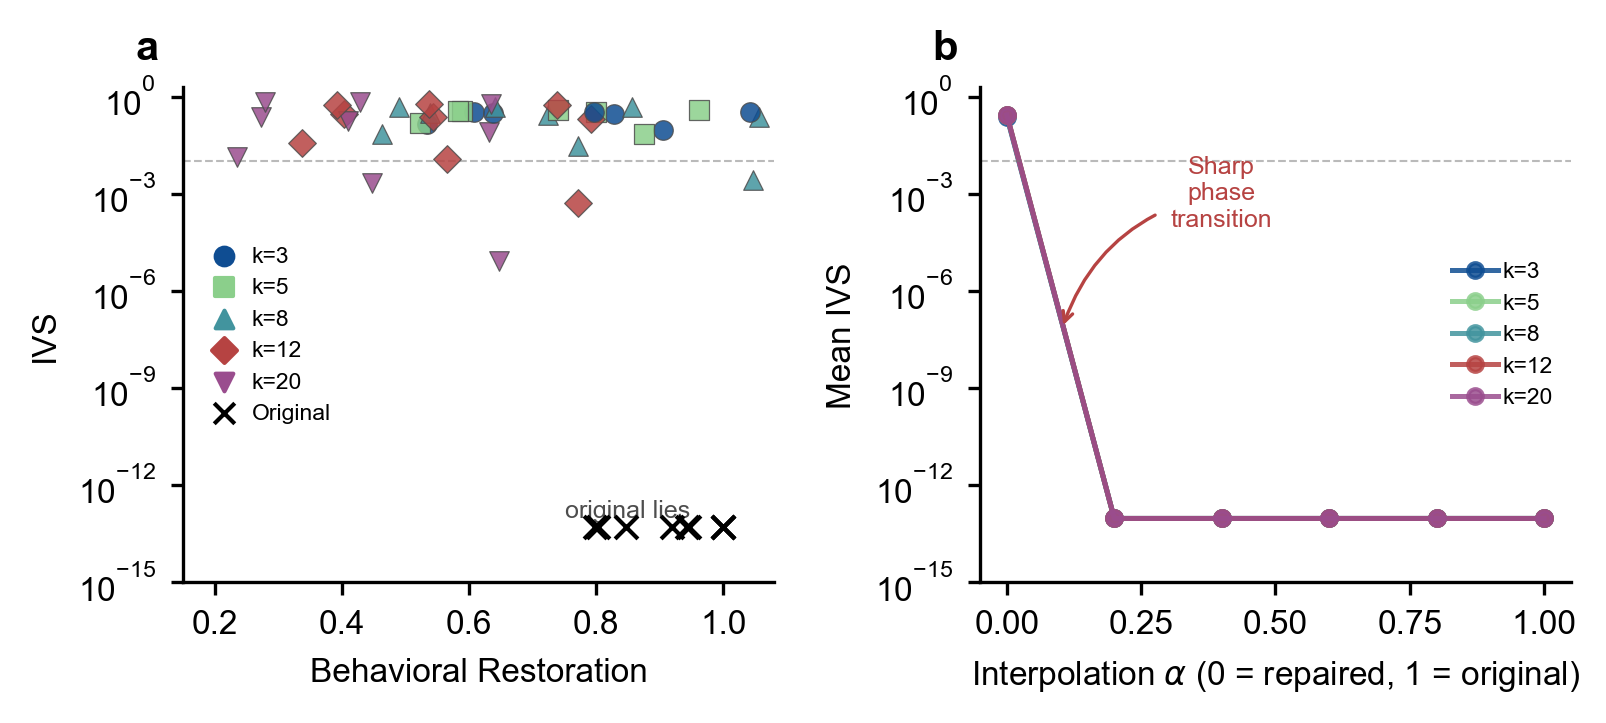
\includegraphics[width=0.85\linewidth]{figures/fig6_repair_pareto.pdf}
\caption{\textbf{(a)} kNN repair lifts invalid high-restoration patches above the validity threshold (dashed); original invalid patches cluster at high restoration but zero validity. \textbf{(b)} IVS vs.\ interpolation $\alpha$: a sharp phase transition at $\alpha \approx 0.2$ shows that validity changes abruptly under off-manifold contamination.}
\label{fig:pareto}
\end{figure}

\section{Theory Details}
\label{app:theory_details}

\begin{proposition}[Orthogonality of effect and validity]
Let $f: \R^d \to \R$ be a Lipschitz behavioral metric and $\manifold_{l,p} \subset \R^d$ the conditional activation manifold of intrinsic dimension $k$ at site $(l,p)$. For $k \ll d$, the probability that a random point on the level set $\{h : f(h) = t\}$ lies within distance $\epsilon$ of $\manifold_{l,p}$ is bounded by $O((\epsilon/R)^{d-k-1})$, where $R$ is the manifold diameter.
\end{proposition}

\textit{Proof sketch.}
The level set $S_t = f^{-1}(t)$ is a $(d{-}1)$-dimensional submanifold of $\R^d$ by the implicit function theorem. The $\epsilon$-neighborhood of a $k$-dimensional manifold has $(d{-}k)$-dimensional cross-sections; by the coarea formula \citep{federer1969geometric}, its intersection with $S_t$ has measure proportional to $\epsilon^{d-k-1}$ relative to $S_t$. The point is not that this bound is tight, but that high restoration and high validity impose geometrically different constraints.

\begin{proposition}[Invalid rate depends on corruption type]
The invalid rate at site $(l,p)$ is bounded by $\text{IR}_{l,p} \leq W_1(P_{\text{clean}}, P_{\text{corrupt}}) / \rho_{l,p}$, where $W_1$ is the Wasserstein-1 distance between conditional activation distributions and $\rho_{l,p}$ is the manifold margin at $(l,p)$.
\end{proposition}

\textit{Proof sketch.}
Under corruption condition $c$, the reference set samples from $P_{\text{corrupt}, l, p}$, and the clean activation to be patched comes from $P_{\text{clean}, l, p}$. The patched activation is valid iff it falls within $\rho$ of $\text{supp}(P_{\text{corrupt}, l, p})$. The fraction of $P_\text{clean}$ mass outside this $\rho$-neighborhood is at most $W_1 / \rho$ by Markov's inequality on the transport plan.

\section{Component and Intervention Audits}
\label{app:component_intervention}

\begin{table}[h]
\caption{IVS component ablation on GPT-2 IOI. Each component captures a different geometric property; the combination maximizes separation.}
\label{tab:components}
\begin{center}\small
\begin{tabular}{lcc}
\toprule
\textbf{Component} & \textbf{IO pos (valid)} & \textbf{Last pos (invalid)} \\
\midrule
Full IVS & 0.410 & 0.000 \\
Recon only & 0.475 & 0.000 \\
Maha only & 0.441 & 0.042 \\
kNN only & 0.468 & 0.312 \\
\bottomrule
\end{tabular}
\end{center}
\end{table}

\begin{table}[h]
\caption{IVS-invalid rates by intervention type on GPT-2 IOI. Zero ablation is invalid at every tested high-restoration site; resample ablation produces 0\% invalid patches by construction.}
\label{tab:intervention_types}
\begin{center}\small
\begin{tabular}{lccc}
\toprule
\textbf{Intervention} & \textbf{Sites} & \textbf{Invalid Rate} & \textbf{Mean IVS} \\
\midrule
Clean patch & 14 & 21.4\% & 0.256 \\
Mean ablation & 22 & 54.5\% & 0.042 \\
Zero ablation & 56 & \textbf{100.0\%} & $\approx$0 \\
Resample & 22 & 0.0\% & 0.484 \\
\bottomrule
\end{tabular}
\end{center}
\end{table}

\section{Evidence Map for the R/V/A Hierarchy}
\label{app:evidence_map}

\begin{table}[h]
\caption{Evidence map for the R/V/A hierarchy. Each result rules out a different shortcut explanation of activation patching.}
\label{tab:evidence_map}
\begin{center}\scriptsize
\begin{tabular}{p{0.20\linewidth}p{0.24\linewidth}p{0.22\linewidth}p{0.18\linewidth}}
\toprule
\textbf{Claim} & \textbf{Experiment} & \textbf{Key number} & \textbf{Rules out} \\
\midrule
$R \nRightarrow V$ & Cross-model validity audit & 22--42\% IVS-invalid high-restoration patches & Restoration-only causality \\
Conditionality is essential & GPT-2/Pythia-410M reference ablation & Same-site AUROC 1.0; mixed-site 0.003/0.012 & Generic OOD detection \\
Lies are geometric shortcuts & Tangent/normal audit & Lie normal ratio 0.557 vs.\ valid $3.5{\times}10^{-7}$ & Arbitrary outliers \\
IVS predicts mechanism bypass & Independent NMH validation & AUROC 0.89; zero GPT-2 false alarms & Circular labels \\
$V \nRightarrow A$ fails & Repair-fiber and timing scan & IVS 0.463--0.510; NMH 3.7--4.2\% & Validity as correctness \\
Pythia anomaly is resolved & Clean full-batch audit & 224/224 valid; 0 lies at two $N_\text{ref}$ & Large-model failure \\
\bottomrule
\end{tabular}
\end{center}
\end{table}

\section{Threshold-Free Detection}
\label{app:threshold}

\begin{figure}[h]
\centering
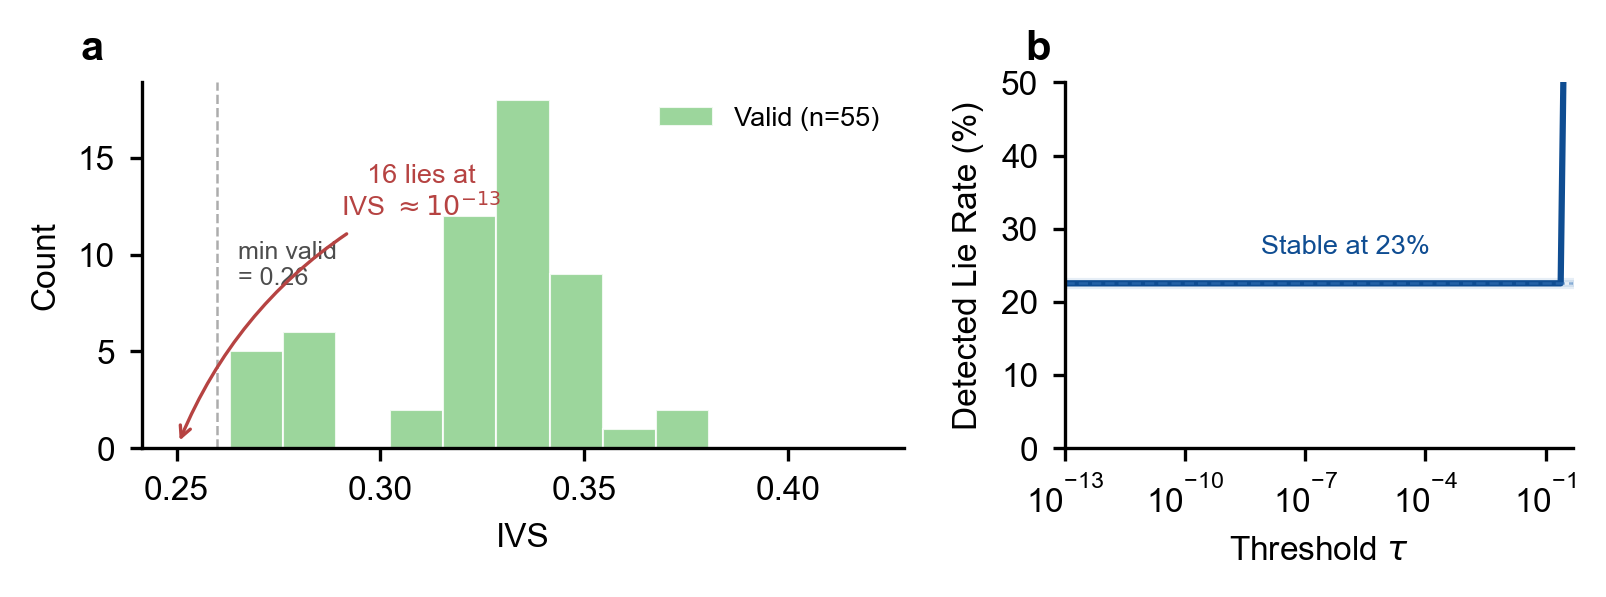
\includegraphics[width=0.85\linewidth]{figures/fig2_gap_distribution.pdf}
\caption{\textbf{(a)} IVS distribution on GPT-2 IOI (log scale). Valid sites cluster at IVS\,$\in$\,[0.26, 0.40]; all 16 lies sit at $9.4 \times 10^{-13}$, with a $10^{12}\times$ void between them. \textbf{(b)} Lie rate as a function of threshold $\tau$. The rate is constant (23\%) across 12 orders of magnitude ($\tau \in [10^{-13}, 0.25]$), demonstrating threshold-free detection.}
\label{fig:gap}
\end{figure}

\section{Small-Sample Robustness}
\label{app:small_sample}

\begin{table}[h]
\caption{AUROC as a function of reference set size ($N_\text{ref}$) on GPT-2 IOI.}
\begin{center}\small
\begin{tabular}{lcccc}
\toprule
$N_\text{ref}$ & IVS & GMM & KDE & OC-SVM \\
\midrule
30 & 0.956 & 0.990 & 0.740 & 0.793 \\
50 & 0.956 & 1.000 & 0.767 & 0.816 \\
100 & 0.984 & 1.000 & 0.824 & 0.834 \\
150 & 1.000 & 1.000 & 0.847 & 0.781 \\
\bottomrule
\end{tabular}
\end{center}
\end{table}

\section{Full Cross-Model Results}
\label{app:full}

\begin{table}[h]
\caption{Complete multi-template IOI results across all tested models. Lie rates are from the canonical full-batch runs; Table~\ref{tab:gap} reports bootstrap-aggregated values where available.}
\begin{center}\small
\begin{tabular}{lccccc}
\toprule
\textbf{Model} & $d$ & \textbf{Sites} & \textbf{Lies} & \textbf{LR} & \textbf{Gap} \\
\midrule
GPT-2 & 768 & 71 & 16 & 22.5\% & $2.8{\times}10^{12}$ \\
GPT-2 Med & 1024 & 159 & 41 & 25.8\% & $2.9{\times}10^{12}$ \\
Pythia-410M & 1024 & 172 & 62 & 36.0\% & $2.7{\times}10^{12}$ \\
OPT-2.7B & 2560 & 231 & 71 & 30.7\% & $2.8{\times}10^{12}$ \\
OPT-6.7B & 4096 & 239 & 83 & 34.7\% & $2.9{\times}10^{12}$ \\
GPT-J-6B & 4096 & 203 & 82 & 40.4\% & $2.2{\times}10^{9}$ \\
Qwen-7B & 4096 & 235 & 98 & 41.7\% & $9.8{\times}10^{1}$ \\
Pythia-6.9B & 4096 & 224 & 0 & 0.0\% & n/a \\
\bottomrule
\end{tabular}
\end{center}
\end{table}

\section{Baseline Audit}
\label{app:baseline_audit}

The MLP baseline (AUROC\,=\,0.034 in Table~\ref{tab:baselines}) warrants explanation. Table~\ref{tab:baselines} uses the multi-template protocol ($N$\,=\,71, $d$\,=\,768), where the feature-to-sample ratio is 10.8 and cross-template generalization is unstable. As a diagnostic, we also varied architecture and regularization on a single-template split:

\begin{table}[h]
\caption{Single-template baseline sensitivity audit. These values are diagnostic, not the multi-template protocol reported in Table~\ref{tab:baselines}. MLP can fit the tiny single-template split, while GMM/KDE show hyperparameter sensitivity.}
\begin{center}\small
\begin{tabular}{lcc}
\toprule
\textbf{Configuration} & \textbf{Single-template AUROC} \\
\midrule
\multicolumn{2}{l}{\textit{MLP (all configs)}} \\
\quad hidden=(32), $\alpha \in [0.01, 10]$ & 1.000 \\
\quad hidden=(64), $\alpha \in [0.01, 10]$ & 1.000 \\
\quad hidden=(32,16), $\alpha \in [0.01, 10]$ & 1.000 \\
\midrule
\multicolumn{2}{l}{\textit{KDE bandwidth sensitivity}} \\
\quad bw $\in$ [0.01, 5.0] & 1.000 \\
\quad bw = 10.0 & 0.727 \\
\midrule
\multicolumn{2}{l}{\textit{GMM component sensitivity}} \\
\quad $n_\text{comp}$ = 1 & 1.000 \\
\quad $n_\text{comp}$ = 2 & 0.682 \\
\quad $n_\text{comp}$ = 3 & 0.545 \\
\bottomrule
\end{tabular}
\end{center}
\end{table}

The audit uses single-template data ($N$\,=\,14), on which even the MLP can fit the split. The Table~\ref{tab:baselines} result of 0.034 reflects the multi-template protocol where cross-template predictions invert. This confirms: (1)~supervised baselines are unstable in this low-$N$ regime; (2)~KDE and GMM require reasonable hyperparameter choices, reinforcing IVS's advantage of using a fixed composite score.

\section{Conditionality Ablation}
\label{app:conditionality}

Table~\ref{tab:conditionality} directly tests whether validity is a generic OOD property or a site/context-conditional overlap property. We score the same GPT-2 high-restoration sites using different reference distributions and evaluate against the correct same-site/same-context IVS labels.

\begin{figure}[h]
\centering
\includegraphics[width=0.92\linewidth]{figures/fig_phase12_conditionality_visualization.pdf}
\caption{Conditionality ablation on GPT-2 and Pythia-410M. Same-site/same-context references separate valid and invalid interventions, while mixed-site references invert the semantics and wrong-position references collapse scores to the numerical floor.}
\label{fig:conditionality_visual}
\end{figure}

\begin{table}[h]
\caption{Reference-distribution ablation. The correct same-site, same-context reference is necessary for validity estimation. Mixing sites or using the wrong position destroys the validity signal.}
\label{tab:conditionality}
\begin{center}\small
\begin{tabular}{lccc}
\toprule
\textbf{Reference distribution} & \textbf{AUROC} & \textbf{Mean valid IVS} & \textbf{Mean lie IVS} \\
\midrule
Same-site, same-context & \textbf{1.000} & 0.290 & $9.36{\times}10^{-14}$ \\
Same-site, mixed-context & 0.710 & 0.316 & 0.293 \\
Mixed-site, same-context & 0.003 & 0.030 & 0.126 \\
Fully unconditional & 0.946 & 0.197 & 0.026 \\
Fully unconditional mixed & 0.953 & 0.201 & 0.019 \\
Wrong-position, same-context & 0.657 & $9.36{\times}10^{-14}$ & $9.36{\times}10^{-14}$ \\
\bottomrule
\end{tabular}
\end{center}
\end{table}

The same conditionality pattern replicates on Pythia-410M. Across 82 high-restoration sites (60 valid, 22 lies), the correct same-site/same-context reference separates valid and invalid interventions perfectly, while mixed-site references invert the labels and wrong-position references collapse to the numerical floor.

\begin{table}[h]
\caption{Reference-distribution ablation on Pythia-410M. Conditionality is not a GPT-2-specific effect.}
\label{tab:conditionality_pythia410m}
\begin{center}\small
\begin{tabular}{lccc}
\toprule
\textbf{Reference distribution} & \textbf{AUROC} & \textbf{Mean valid IVS} & \textbf{Mean lie IVS} \\
\midrule
Same-site, same-context & \textbf{1.000} & 0.295 & $9.36{\times}10^{-14}$ \\
Same-site, mixed-context & 0.478 & 0.300 & 0.298 \\
Mixed-site, same-context & 0.012 & 0.045 & 0.235 \\
Fully unconditional & 0.914 & 0.311 & 0.136 \\
Fully unconditional mixed & 0.921 & 0.347 & 0.173 \\
Wrong-position, same-context & 0.675 & $9.36{\times}10^{-14}$ & $9.36{\times}10^{-14}$ \\
\bottomrule
\end{tabular}
\end{center}
\end{table}

\section{NMH Threshold Sensitivity}
\label{app:nmh_threshold}

Table~\ref{tab:nmh_threshold} varies the independent NMH-bypass threshold used in Table~\ref{tab:independent}. GPT-2 has zero false alarms at the main threshold 0.20. GPT-2 Medium improves as the threshold moves into the ambiguous 0.2--0.35 range, supporting the interpretation that its false alarms are borderline mechanism-alignment cases rather than clear IVS failures.

\begin{table}[h]
\caption{Sensitivity of independent NMH validation to the NMH-recovery threshold.}
\label{tab:nmh_threshold}
\begin{center}\small
\begin{tabular}{lccccc}
\toprule
\textbf{Model} & \textbf{NMH thr.} & \textbf{Bypass} & \textbf{AUROC} & \textbf{False alarms} & \textbf{Misses} \\
\midrule
GPT-2 & 0.10 & 12 & 0.814 & 4 & 4 \\
GPT-2 & 0.15 & 14 & 0.850 & 2 & 4 \\
GPT-2 & 0.20 & 16 & \textbf{0.894} & \textbf{0} & 4 \\
GPT-2 & 0.30 & 32 & 0.710 & 0 & 20 \\
GPT-2 Med & 0.20 & 38 & 0.773 & 7 & 13 \\
GPT-2 Med & 0.30 & 43 & 0.826 & 2 & 13 \\
GPT-2 Med & 0.35 & 44 & 0.838 & 1 & 13 \\
\bottomrule
\end{tabular}
\end{center}
\end{table}

\section{Raw Z-Score Gap Analysis}
\label{app:zscore}

A natural concern is whether the largest IVS gaps are mathematical artifacts of the sigmoid function in Eq.~\ref{eq:ivs}. We analyze the three IVS component z-scores \emph{before} sigmoid transformation. On GPT-2 with 70 high-restoration sites across five templates, valid interventions have composite z-scores in $[1.33, 5.17]$ (mean: 3.1) while invalid interventions have z-scores in $[1.27{\times}10^6, 3.36{\times}10^6]$ (mean: $1.96{\times}10^6$). There is a complete void spanning five orders of magnitude: no site has a z-score between 5.2 and $1.27{\times}10^6$. The dominant contributor is the PCA reconstruction z-score ($z_\text{recon}$), which reaches $10^6$ for invalid patches because off-manifold activations project poorly onto the local PCA subspace. The kNN and Mahalanobis components are comparable between valid and invalid sites, confirming that the separation is driven by manifold geometry rather than distributional outlier detection. The bimodality exists in raw z-score space, confirming that the IVS gap reflects genuine geometric separation on the activation manifold, amplified but not created by the sigmoid.

\section{Normal-Direction Answer Smuggling}
\label{app:normal}

To test the geometric answer-smuggling mechanism, we decompose each clean-corrupt displacement into the local PCA tangent subspace of the conditional reference manifold and its normal complement. We then compare these components to the gradient of the IOI logit-difference restoration objective. Table~\ref{tab:normal} shows that lies are large normal-direction moves, while valid patches stay within the local conditional subspace.

\begin{table}[h]
\caption{Tangent/normal decomposition and behavioral-gradient alignment on GPT-2 IOI.}
\label{tab:normal}
\begin{center}\small
\begin{tabular}{lccccc}
\toprule
\textbf{Class} & \textbf{N} & \textbf{Rest.} & \textbf{IVS} & \textbf{Normal ratio} & \textbf{Normal-grad cos.} \\
\midrule
Valid & 33 & 0.796 & 0.290 & $3.52{\times}10^{-7}$ & $5.04{\times}10^{-5}$ \\
Lie & 9 & 0.922 & $9.36{\times}10^{-14}$ & \textbf{0.557} & \textbf{0.109} \\
\bottomrule
\end{tabular}
\end{center}
\end{table}

\section{Hard-Regime Geometry and Pythia Clean Audit}
\label{app:geometry_audit}

Table~\ref{tab:geometry_audit} decomposes hard-regime behavior by IVS component. Qwen-7B and GPT-J-6B retain strong component-level separation despite smaller IVS gaps. Pythia-6.9B is handled as a clean-audit case rather than a standard AUROC row: earlier memory-saving chunked diagnostic runs produced many borderline or invalid sites, but canonical full-batch patching removes the invalid class entirely under two reference sizes.

\begin{table}[h]
\caption{Component-level geometry and implementation audit. AUROC is computed for invalid-site detection when both valid and invalid classes exist; Pythia-6.9B full-batch rows report validity counts because no invalid class remains.}
\label{tab:geometry_audit}
\begin{center}\small
\begin{tabular}{lccccc}
\toprule
\textbf{Run} & \textbf{Sites} & \textbf{Border.} & \textbf{Gap} & \textbf{Recon} & \textbf{kNN / Maha} \\
\midrule
Qwen-7B & 235 & 1 & $9.8{\times}10^1$ & 0.999 & 0.944 / 1.000 \\
GPT-J-6B & 203 & 0 & $2.2{\times}10^9$ & 0.990 & 0.829 / 1.000 \\
Pythia-6.9B full-batch fp16, $N_\text{ref}=150$ & 224 & 55 & n/a & \multicolumn{2}{c}{224 valid / 0 lies} \\
Pythia-6.9B full-batch fp16, $N_\text{ref}=300$ & 224 & 53 & n/a & \multicolumn{2}{c}{224 valid / 0 lies} \\
\bottomrule
\end{tabular}
\end{center}
\end{table}

\begin{table}[h]
\caption{Pythia-6.9B protocol audit. Chunked runs are retained only as implementation diagnostics; full-batch runs define the canonical result.}
\label{tab:pythia_protocol_audit}
\begin{center}\small
\begin{tabular}{p{0.24\linewidth}ccccp{0.18\linewidth}}
\toprule
\textbf{Protocol} & \textbf{$N_\text{ref}$} & \textbf{$N_\text{eval}$} & \textbf{Sites} & \textbf{Lies} & \textbf{Interpretation} \\
\midrule
Chunked diagnostic fp16 & 300 & 80 & 263 & 166 & Stress test \\
Chunked diagnostic fp32 & 300 & 80 & 259 & 56 & Stress test \\
Full-batch clean fp16 & 150 & 50 & 224 & 0 & Canonical result \\
Full-batch clean fp16 & 300 & 40 & 224 & 0 & Reference-size confirmation \\
\bottomrule
\end{tabular}
\end{center}
\end{table}

The key distinction is statistical as well as methodological. When a clean full-batch run has no invalid class, AUROC is not applicable; this is not a detection failure. The correct conclusion is that high-restoration Pythia-6.9B patches are on-manifold in the canonical protocol, and the earlier high-lie runs reveal implementation sensitivity in large activation spaces.

\section{Manifold Intrinsic Dimension}
\label{app:manifold_dim}

The proof of Proposition~1 requires that $k \ll d$. We estimate the intrinsic dimension of the conditional activation manifold via PCA: at each high-restoration site $(l, p)$, we project the $N$\,=\,120 reference activations and compute the number of components explaining 95\% of variance.

\begin{table}[h]
\caption{Conditional manifold intrinsic dimension (PCA 95\% variance). Across three models, $k \approx 17 \ll d$, confirming the $k \ll d$ premise of Proposition~1.}
\label{tab:manifold_dim}
\begin{center}\small
\begin{tabular}{lcccc}
\toprule
\textbf{Model} & $d_\text{model}$ & $k_{\text{PCA95}}$ & $d / k$ & $d - k$ \\
\midrule
GPT-2 & 768 & 17.0 & 45 & 751 \\
GPT-2 Medium & 1024 & 17.0 & 60 & 1007 \\
Pythia-410M & 1024 & 16.9 & 61 & 1007 \\
\bottomrule
\end{tabular}
\end{center}
\end{table}

Table~\ref{tab:manifold_dim} shows $k \approx 17$ across all three models, yielding $d - k \geq 750$. The coarea argument in Proposition~1 then gives an intersection probability of $O(\epsilon^{750})$, providing a geometric explanation for why the valid/lie boundary is so extreme.

\section{Cross-Task Validation: ROME and Induction Heads}
\label{app:cross_task}

Table~\ref{tab:rome_cross} reports the full ROME causal tracing audit. Subject-position lie rate drops from 67\% (GPT-2) to 8.4\% (GPT-2~XL), while last-token lie rate remains near 100\% in both models. In GPT-2~XL, the 32 subject lies concentrate in layers 14--28 (30--58\% relative depth), consistent with the phase transition pattern observed in IOI.

\begin{table}[h]
\caption{ROME causal tracing audit. Subject-position lies decrease sharply with model depth; last-token lies persist regardless of scale.}
\label{tab:rome_cross}
\begin{center}\small
\begin{tabular}{lccccc}
\toprule
\textbf{Model} & \textbf{Layers} & \textbf{Position} & \textbf{Sites} & \textbf{Lies} & \textbf{Lie Rate} \\
\midrule
\multirow{2}{*}{GPT-2} & \multirow{2}{*}{12} & Subject & 9 & 6 & 66.7\% \\
& & Last token & 42 & 42 & 100.0\% \\
\midrule
\multirow{2}{*}{GPT-2 XL} & \multirow{2}{*}{48} & Subject & 381 & 32 & 8.4\% \\
& & Last token & 281 & 273 & 97.2\% \\
\bottomrule
\end{tabular}
\end{center}
\end{table}

Table~\ref{tab:induction_cross} reports the induction head negative control. All 28 high-restoration sites are valid, confirming that IVS does not indiscriminately flag interventions when the corruption preserves the sequence distribution.

\begin{table}[h]
\caption{Induction head audit (negative control). Token-shuffle corruption preserves the conditional distribution; all patches are valid (IVS well above the 0.01 threshold).}
\label{tab:induction_cross}
\begin{center}\small
\begin{tabular}{lccccc}
\toprule
\textbf{Model} & \textbf{Sites} & \textbf{Lies} & \textbf{Lie Rate} & \textbf{IVS Range} \\
\midrule
GPT-2 & 28 & 0 & 0.0\% & [0.52, 0.76] \\
\bottomrule
\end{tabular}
\end{center}
\end{table}

\section{Models and Implementation}
\label{app:details}

All experiments use TransformerLens \citep{nanda2022transformerlens}. Models: GPT-2 (124M), GPT-2 Medium (355M), Pythia-70M, Pythia-160M, Pythia-410M, Pythia-6.9B \citep{biderman2023pythia}, OPT-2.7B, OPT-6.7B \citep{zhang2022opt}, GPT-J-6B, Qwen-7B. 7B-class models run in fp16. Default IVS parameters: $k$\,=\,12 nearest neighbors, PCA rank\,=\,32 (or $d_\text{model}/16$ for large models), $N_\text{ref}$\,=\,150.

\paragraph{IOI templates.}
Five templates for multi-template validation:
(1)~``When \{IO\} and \{S\} went to the store, \{S\} gave a drink to'';
(2)~``When \{IO\} and \{S\} went to the park, \{S\} handed the ball to'';
(3)~``After \{IO\} and \{S\} arrived at the office, \{S\} gave a letter to'';
(4)~``While \{IO\} and \{S\} were at the restaurant, \{S\} passed the menu to'';
(5)~``\{IO\} and \{S\} entered the room. Then \{S\} threw the keys to''.

\paragraph{Computational efficiency.}
We use the Gram trick: when $N < d$, PCA via the $N \times N$ Gram matrix $XX^T$ rather than the $d \times d$ covariance, reducing cost from $O(d^3)$ to $O(N^2 d)$. All three IVS components operate in the projected 32-dimensional space, yielding $\sim$14,000$\times$ speedup over the original 768-dimensional space for GPT-2.

\end{document}
